%% LyX 2.0.5.1 created this file.  For more info, see http://www.lyx.org/.
%% Do not edit unless you really know what you are doing.
\documentclass{article}\usepackage{graphicx, color}
%% maxwidth is the original width if it is less than linewidth
%% otherwise use linewidth (to make sure the graphics do not exceed the margin)
\makeatletter
\def\maxwidth{ %
  \ifdim\Gin@nat@width>\linewidth
    \linewidth
  \else
    \Gin@nat@width
  \fi
}
\makeatother

\IfFileExists{upquote.sty}{\usepackage{upquote}}{}
\definecolor{fgcolor}{rgb}{0.2, 0.2, 0.2}
\newcommand{\hlnumber}[1]{\textcolor[rgb]{0,0,0}{#1}}%
\newcommand{\hlfunctioncall}[1]{\textcolor[rgb]{0.501960784313725,0,0.329411764705882}{\textbf{#1}}}%
\newcommand{\hlstring}[1]{\textcolor[rgb]{0.6,0.6,1}{#1}}%
\newcommand{\hlkeyword}[1]{\textcolor[rgb]{0,0,0}{\textbf{#1}}}%
\newcommand{\hlargument}[1]{\textcolor[rgb]{0.690196078431373,0.250980392156863,0.0196078431372549}{#1}}%
\newcommand{\hlcomment}[1]{\textcolor[rgb]{0.180392156862745,0.6,0.341176470588235}{#1}}%
\newcommand{\hlroxygencomment}[1]{\textcolor[rgb]{0.43921568627451,0.47843137254902,0.701960784313725}{#1}}%
\newcommand{\hlformalargs}[1]{\textcolor[rgb]{0.690196078431373,0.250980392156863,0.0196078431372549}{#1}}%
\newcommand{\hleqformalargs}[1]{\textcolor[rgb]{0.690196078431373,0.250980392156863,0.0196078431372549}{#1}}%
\newcommand{\hlassignement}[1]{\textcolor[rgb]{0,0,0}{\textbf{#1}}}%
\newcommand{\hlpackage}[1]{\textcolor[rgb]{0.588235294117647,0.709803921568627,0.145098039215686}{#1}}%
\newcommand{\hlslot}[1]{\textit{#1}}%
\newcommand{\hlsymbol}[1]{\textcolor[rgb]{0,0,0}{#1}}%
\newcommand{\hlprompt}[1]{\textcolor[rgb]{0.2,0.2,0.2}{#1}}%

\usepackage{framed}
\makeatletter
\newenvironment{kframe}{%
 \def\at@end@of@kframe{}%
 \ifinner\ifhmode%
  \def\at@end@of@kframe{\end{minipage}}%
  \begin{minipage}{\columnwidth}%
 \fi\fi%
 \def\FrameCommand##1{\hskip\@totalleftmargin \hskip-\fboxsep
 \colorbox{shadecolor}{##1}\hskip-\fboxsep
     % There is no \\@totalrightmargin, so:
     \hskip-\linewidth \hskip-\@totalleftmargin \hskip\columnwidth}%
 \MakeFramed {\advance\hsize-\width
   \@totalleftmargin\z@ \linewidth\hsize
   \@setminipage}}%
 {\par\unskip\endMakeFramed%
 \at@end@of@kframe}
\makeatother

\definecolor{shadecolor}{rgb}{.97, .97, .97}
\definecolor{messagecolor}{rgb}{0, 0, 0}
\definecolor{warningcolor}{rgb}{1, 0, 1}
\definecolor{errorcolor}{rgb}{1, 0, 0}
\newenvironment{knitrout}{}{} % an empty environment to be redefined in TeX

\usepackage{alltt}
\usepackage[sc]{mathpazo}
\usepackage{geometry}
\geometry{verbose,tmargin=2.5cm,bmargin=2.5cm,lmargin=2.5cm,rmargin=2.5cm}
\setcounter{secnumdepth}{2}
\setcounter{tocdepth}{2}
\usepackage{url}
\usepackage[unicode=true,pdfusetitle,
 bookmarks=true,bookmarksnumbered=true,bookmarksopen=true,bookmarksopenlevel=2,
 breaklinks=false,pdfborder={0 0 1},backref=false,colorlinks=false]
 {hyperref}
\hypersetup{
 pdfstartview={XYZ null null 1}}
\usepackage{breakurl}
\begin{document}





\title{Stat 2025- HW 4}
\author{Michael Discenza}

\maketitle

To start out, we plot the distribution of the response variable, count.  We also note that as a count, it takes only integers values.  This provides us with the insight that we might be best served by using poisson regression or negative binomial regression.
\begin{knitrout}
\definecolor{shadecolor}{rgb}{0.969, 0.969, 0.969}\color{fgcolor}\begin{kframe}
\begin{alltt}
\hlfunctioncall{library}(boot)
\hlfunctioncall{library}(pscl)
\hlfunctioncall{library}(VGAM)
\hlfunctioncall{library}(MASS)
fish <- \hlfunctioncall{read.table}(\hlfunctioncall{url}(\hlstring{"http://www.stat.columbia.edu/~madigan/W2025/data/fish.csv"}), sep = \hlstring{","}, 
    header = TRUE)
fish <- \hlfunctioncall{as.data.frame}(\hlfunctioncall{cbind}(fish$count, fish$child, fish$camper, fish$persons))
\hlfunctioncall{colnames}(fish) <- \hlfunctioncall{c}(\hlstring{"count"}, \hlstring{"child"}, \hlstring{"camper"}, \hlstring{"persons"})
\hlfunctioncall{plot}(\hlfunctioncall{density}(fish$count), main = \hlstring{"Response Varible Density"})
\hlfunctioncall{plot}(\hlfunctioncall{density}(\hlfunctioncall{subset}(fish$count, (fish$count > 0 & fish$count < 100))), main = \hlstring{"Response Varible \hlfunctioncall{Density} (with no zeros)"})
\end{alltt}
\end{kframe}

{\centering 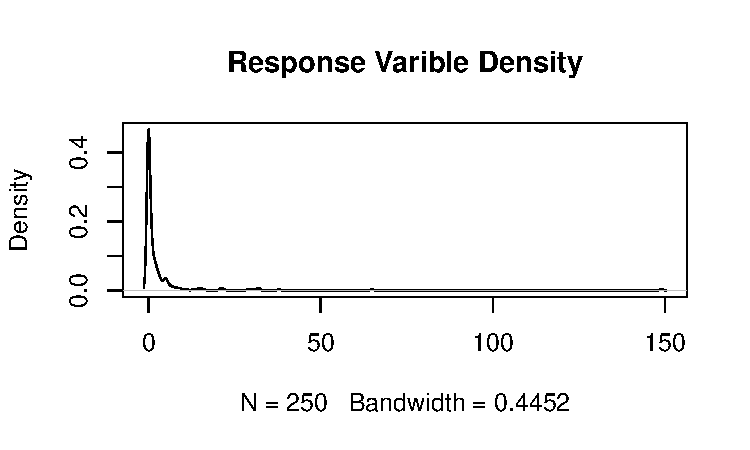
\includegraphics[width=\maxwidth]{figure/minimal-start1} 
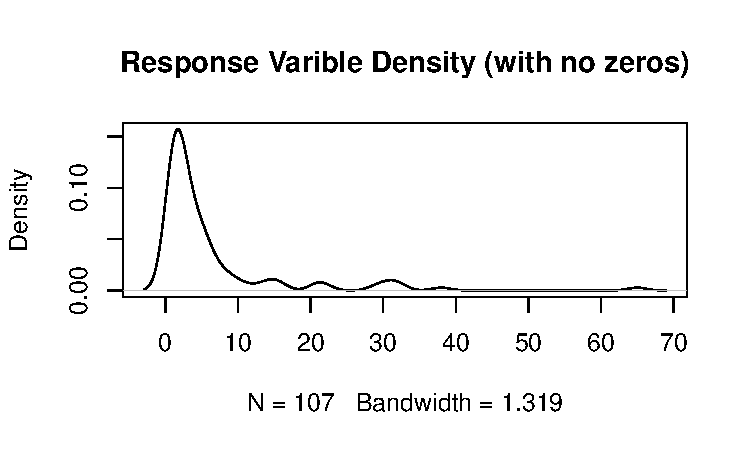
\includegraphics[width=\maxwidth]{figure/minimal-start2} 

}



\end{knitrout}

In the first desnity plot, we see that the majority of responses are around 0.  We can again plot the data, this time subsetting it so that we do not plot zeros or values that are greater than 100.  In that second plot, we see that the values are again highly concentrated around between 1 and 10.  Before proceeding, we should also check for the presence of two common problems in the data that we might encounter when fitting a Poisson Regression model- overdispersion and zero inflation, the latter of which seems a first glance to be an issue.

\begin{knitrout}
\definecolor{shadecolor}{rgb}{0.969, 0.969, 0.969}\color{fgcolor}\begin{kframe}
\begin{alltt}
\hlfunctioncall{length}(\hlfunctioncall{subset}(fish$count, fish$count == 0))
\end{alltt}
\begin{verbatim}
## [1] 142
\end{verbatim}
\begin{alltt}
\hlfunctioncall{mean}(fish$count)
\end{alltt}
\begin{verbatim}
## [1] 3.296
\end{verbatim}
\begin{alltt}
\hlfunctioncall{sqrt}(\hlfunctioncall{var}(fish$count))
\end{alltt}
\begin{verbatim}
## [1] 11.64
\end{verbatim}
\begin{alltt}
fish_no_zero <- \hlfunctioncall{subset}(fish$count, fish$count != 0)
\hlfunctioncall{mean}(fish_no_zero)
\end{alltt}
\begin{verbatim}
## [1] 7.63
\end{verbatim}
\begin{alltt}
\hlfunctioncall{var}(fish_no_zero)
\end{alltt}
\begin{verbatim}
## [1] 281.7
\end{verbatim}
\end{kframe}
\end{knitrout}

We see that we have a problem with both overdispersion and zero inflation.  Looking at the mean and variance for the distribution without zeros, we see that there is still a problem with overdispersion and that we should fit zero-inflated and zero-altered models, to either Poisson Model, where we correct the standard errors using a quasi-GLM model, or a negative binomial model.  

Before fitting the models, we make a structure that will allow us to track the performance of each of the models and define paramenters that we will use for cross validation of the models.  It is important to note that we had to redfine the cost function of the CV function to round the fitted values to the nearest whole number because it does not make sense to have non-integer fitted values for counts.

\begin{knitrout}
\definecolor{shadecolor}{rgb}{0.969, 0.969, 0.969}\color{fgcolor}\begin{kframe}
\begin{alltt}
model <- \hlfunctioncall{rep}(NA, 6)
AIC <- \hlfunctioncall{rep}(NA, 6)
CV.PredictionError <- \hlfunctioncall{rep}(NA, 6)
k_fold <- 50
costf <- \hlfunctioncall{function}(r, pi = 0) \hlfunctioncall{mean}((r - \hlfunctioncall{round}(pi))^2)
costfb <- \hlfunctioncall{function}(r, pi = 0) \hlfunctioncall{mean}((r - pi)^2)
\end{alltt}
\end{kframe}
\end{knitrout}


The non-zero-altered version of the quasi-Poisson.  Note for this model, we cannot calculate an AIC value
\begin{knitrout}
\definecolor{shadecolor}{rgb}{0.969, 0.969, 0.969}\color{fgcolor}\begin{kframe}
\begin{alltt}
model[1] <- \hlstring{"Unaltered Poisson"}
m1 <- \hlfunctioncall{glm}(count ~ child + camper + persons, data = fish, family = \hlstring{"quasipoisson"})
\hlfunctioncall{summary}(m1)
\end{alltt}
\begin{verbatim}
## 
## Call:
## glm(formula = count ~ child + camper + persons, family = "quasipoisson", 
##     data = fish)
## 
## Deviance Residuals: 
##    Min      1Q  Median      3Q     Max  
## -6.810  -1.443  -0.906  -0.041  16.142  
## 
## Coefficients:
##             Estimate Std. Error t value Pr(>|t|)    
## (Intercept)   -1.982      0.524   -3.78  0.00019 ***
## child         -1.690      0.279   -6.07  4.9e-09 ***
## camper         0.931      0.306    3.04  0.00264 ** 
## persons        1.091      0.135    8.08  2.9e-14 ***
## ---
## Signif. codes:  0 '***' 0.001 '**' 0.01 '*' 0.05 '.' 0.1 ' ' 1 
## 
## (Dispersion parameter for quasipoisson family taken to be 11.83)
## 
##     Null deviance: 2958.4  on 249  degrees of freedom
## Residual deviance: 1337.1  on 246  degrees of freedom
## AIC: NA
## 
## Number of Fisher Scoring iterations: 6
\end{verbatim}
\begin{alltt}
\hlcomment{# leave-one-out cross validation error}
CV.PredictionError[1] <- \hlfunctioncall{cv.glm}(data = fish, glmfit = m1, K = k_fold, cost = costf)$delta[2]
CV.PredictionError[1]
\end{alltt}
\begin{verbatim}
## [1] 104.1
\end{verbatim}
\end{kframe}
\end{knitrout}


Above, we see that the disperssion paramerter is almost 12, much higher than 1, making it unaccepatble to fit using a normal poisson model.  We alo see that all of the three predictors included in the model, so to simplify our analysis going forward, we continue to fit the full model of the three predictors for each different specification of the GLM.

Next we fit a zero-inflated Poisson, ZIP. Though we are unable to fit a quasi-poisson model and adjust for the overdispersion, we could easily adjust our variance of the fitted parameters afterward with the dispersion parameter, but since we are not doing inference with the parameters or fitting confidence intervals in this exercise, that is not necessary.

\begin{knitrout}
\definecolor{shadecolor}{rgb}{0.969, 0.969, 0.969}\color{fgcolor}\begin{kframe}
\begin{alltt}
model[2] <- \hlstring{"Zero-inflated Poisson"}
f1 <- \hlfunctioncall{formula}(count ~ child + camper + persons | child + camper + persons)
zip1 <- \hlfunctioncall{zeroinfl}(f1, dist = \hlstring{"poisson"}, link = \hlstring{"logit"}, data = fish)
\hlfunctioncall{summary}(zip1)
\end{alltt}
\begin{verbatim}
## 
## Call:
## zeroinfl(formula = f1, data = fish, dist = "poisson", link = "logit")
## 
## Pearson residuals:
##     Min      1Q  Median      3Q     Max 
## -3.0544 -0.7434 -0.4428 -0.0756 27.9930 
## 
## Count model coefficients (poisson with log link):
##             Estimate Std. Error z value Pr(>|z|)    
## (Intercept)  -0.7983     0.1708   -4.67  3.0e-06 ***
## child        -1.1367     0.0930  -12.22  < 2e-16 ***
## camper        0.7243     0.0931    7.78  7.5e-15 ***
## persons       0.8290     0.0440   18.86  < 2e-16 ***
## 
## Zero-inflation model coefficients (binomial with logit link):
##             Estimate Std. Error z value Pr(>|z|)    
## (Intercept)    1.664      0.516    3.23   0.0013 ** 
## child          1.905      0.326    5.84  5.2e-09 ***
## camper        -0.834      0.353   -2.36   0.0181 *  
## persons       -0.923      0.199   -4.63  3.6e-06 ***
## ---
## Signif. codes:  0 '***' 0.001 '**' 0.01 '*' 0.05 '.' 0.1 ' ' 1 
## 
## Number of iterations in BFGS optimization: 14 
## Log-likelihood: -753 on 8 Df
\end{verbatim}
\begin{alltt}
AIC[2] <- \hlfunctioncall{AIC}(zip1)
AIC[2]
\end{alltt}
\begin{verbatim}
## [1] 1521
\end{verbatim}
\begin{alltt}
\hlcomment{# Leave one out cv error}
cost <- \hlfunctioncall{function}(r, pi = 0) \hlfunctioncall{mean}(\hlfunctioncall{abs}(r - pi) > 0.5)
CV.PredictionError[2] <- \hlfunctioncall{cv.glm}(data = fish, glmfit = zip1, K = k_fold, cost = costf)$delta[2]
CV.PredictionError[2]
\end{alltt}
\begin{verbatim}
## [1] 105.1
\end{verbatim}
\end{kframe}
\end{knitrout}


This model uses the hurdle function and fits a zero-adjusted poisson model instead of zeroinf.  
\begin{knitrout}
\definecolor{shadecolor}{rgb}{0.969, 0.969, 0.969}\color{fgcolor}\begin{kframe}
\begin{alltt}
model[3] <- \hlstring{"Zero-adjusted Poisson"}
H1.P <- \hlfunctioncall{hurdle}(f1, dist = \hlstring{"poisson"}, link = \hlstring{"logit"}, data = fish)
\hlfunctioncall{summary}(H1.P)
\end{alltt}
\begin{verbatim}
## 
## Call:
## hurdle(formula = f1, data = fish, dist = "poisson", link = "logit")
## 
## Pearson residuals:
##     Min      1Q  Median      3Q     Max 
## -3.3223 -0.7358 -0.4646 -0.0601 28.6164 
## 
## Count model coefficients (truncated poisson with log link):
##             Estimate Std. Error z value Pr(>|z|)    
## (Intercept)  -0.8262     0.1723   -4.79  1.6e-06 ***
## child        -1.1390     0.0929  -12.27  < 2e-16 ***
## camper        0.7336     0.0934    7.85  4.1e-15 ***
## persons       0.8348     0.0441   18.95  < 2e-16 ***
## Zero hurdle model coefficients (binomial with logit link):
##             Estimate Std. Error z value Pr(>|z|)    
## (Intercept)   -2.309      0.461   -5.01  5.6e-07 ***
## child         -2.138      0.311   -6.88  5.9e-12 ***
## camper         1.018      0.325    3.14   0.0017 ** 
## persons        1.110      0.191    5.81  6.2e-09 ***
## ---
## Signif. codes:  0 '***' 0.001 '**' 0.01 '*' 0.05 '.' 0.1 ' ' 1 
## 
## Number of iterations in BFGS optimization: 11 
## Log-likelihood: -752 on 8 Df
\end{verbatim}
\begin{alltt}
AIC[3] <- \hlfunctioncall{AIC}(H1.P)
CV.PredictionError[3] <- \hlfunctioncall{cv.glm}(data = fish, glmfit = H1.P, K = k_fold, cost = costf)$delta[2]
CV.PredictionError[3]
\end{alltt}
\begin{verbatim}
## [1] 105.4
\end{verbatim}
\end{kframe}
\end{knitrout}



The next set of models that we fit are negative binomial models instead of poisson, which might serve us better, paritcuarly when using the zeroinf and hurdle functins to fit the mixed models because we are not able to compensate in our variances of fitted parameters for the overdispersion of the response variable without manually scalling the standard deviations.
\begin{knitrout}
\definecolor{shadecolor}{rgb}{0.969, 0.969, 0.969}\color{fgcolor}\begin{kframe}
\begin{alltt}
model[4] <- \hlstring{"Unaltered Negative Binomial"}
m2 <- \hlfunctioncall{glm.nb}(fish$count ~ fish$child + fish$camper + fish$persons, data = fish, link = \hlstring{"log"})
\hlfunctioncall{summary}(m2)
\end{alltt}
\begin{verbatim}
## 
## Call:
## glm.nb(formula = fish$count ~ fish$child + fish$camper + fish$persons, 
##     data = fish, link = "log", init.theta = 0.4635287626)
## 
## Deviance Residuals: 
##    Min      1Q  Median      3Q     Max  
## -1.667  -0.960  -0.659  -0.032   4.943  
## 
## Coefficients:
##              Estimate Std. Error z value Pr(>|z|)    
## (Intercept)    -1.625      0.330   -4.92  8.7e-07 ***
## fish$child     -1.781      0.185   -9.62  < 2e-16 ***
## fish$camper     0.621      0.235    2.65   0.0082 ** 
## fish$persons    1.061      0.114    9.27  < 2e-16 ***
## ---
## Signif. codes:  0 '***' 0.001 '**' 0.01 '*' 0.05 '.' 0.1 ' ' 1 
## 
## (Dispersion parameter for Negative Binomial(0.4635) family taken to be 1)
## 
##     Null deviance: 394.25  on 249  degrees of freedom
## Residual deviance: 210.65  on 246  degrees of freedom
## AIC: 820.4
## 
## Number of Fisher Scoring iterations: 1
## 
## 
##               Theta:  0.4635 
##           Std. Err.:  0.0712 
## 
##  2 x log-likelihood:  -810.4440
\end{verbatim}
\begin{alltt}
AIC[4] <- \hlfunctioncall{AIC}(m2)
CV.PredictionError[4] <- \hlfunctioncall{cv.glm}(data = fish, glmfit = m1, K = k_fold, cost = costf)$delta[2]
CV.PredictionError[4]
\end{alltt}
\begin{verbatim}
## [1] 104.3
\end{verbatim}
\end{kframe}
\end{knitrout}




Here is a zero-inflated negative binomial (ZINB),
\begin{knitrout}
\definecolor{shadecolor}{rgb}{0.969, 0.969, 0.969}\color{fgcolor}\begin{kframe}
\begin{alltt}
model[5] <- \hlstring{"Zero-inflated negative binomial"}
f2 <- \hlfunctioncall{formula}(count ~ child + camper + persons | child + camper + persons)
zip2 <- \hlfunctioncall{zeroinfl}(f2, dist = \hlstring{"negbin"}, link = \hlstring{"logit"}, data = fish)
\hlfunctioncall{summary}(zip2)
\end{alltt}
\begin{verbatim}
## 
## Call:
## zeroinfl(formula = f2, data = fish, dist = "negbin", link = "logit")
## 
## Pearson residuals:
##    Min     1Q Median     3Q    Max 
## -0.718 -0.561 -0.382  0.044 16.164 
## 
## Count model coefficients (negbin with log link):
##             Estimate Std. Error z value Pr(>|z|)    
## (Intercept)   -1.618      0.320   -5.05  4.4e-07 ***
## child         -1.261      0.247   -5.10  3.4e-07 ***
## camper         0.386      0.246    1.57  0.11713    
## persons        1.090      0.112    9.76  < 2e-16 ***
## Log(theta)    -0.593      0.158   -3.75  0.00017 ***
## 
## Zero-inflation model coefficients (binomial with logit link):
##             Estimate Std. Error z value Pr(>|z|)
## (Intercept)  -11.992     64.441   -0.19     0.85
## child         10.952     64.357    0.17     0.86
## camper       -10.770     64.372   -0.17     0.87
## persons        0.290      0.731    0.40     0.69
## ---
## Signif. codes:  0 '***' 0.001 '**' 0.01 '*' 0.05 '.' 0.1 ' ' 1 
## 
## Theta = 0.553 
## Number of iterations in BFGS optimization: 68 
## Log-likelihood: -396 on 9 Df
\end{verbatim}
\begin{alltt}
AIC[5] <- \hlfunctioncall{AIC}(zip2)
CV.PredictionError[5] <- \hlfunctioncall{cv.glm}(data = fish, glmfit = zip2, K = k_fold, cost = costf)$delta[2]
CV.PredictionError[5]
\end{alltt}
\begin{verbatim}
## [1] 104.9
\end{verbatim}
\end{kframe}
\end{knitrout}


Here is a zero-altered negative binomial with the hurdle function
\begin{knitrout}
\definecolor{shadecolor}{rgb}{0.969, 0.969, 0.969}\color{fgcolor}\begin{kframe}
\begin{alltt}
model[6] <- \hlstring{"Zero-altered negative binomial"}
H1.NB <- \hlfunctioncall{hurdle}(f1, dist = \hlstring{"negbin"}, link = \hlstring{"logit"}, data = fish)
\hlfunctioncall{summary}(H1.NB)
\end{alltt}
\begin{verbatim}
## 
## Call:
## hurdle(formula = f1, data = fish, dist = "negbin", link = "logit")
## 
## Pearson residuals:
##     Min      1Q  Median      3Q     Max 
## -0.7277 -0.5159 -0.2594 -0.0329 14.7097 
## 
## Count model coefficients (truncated negbin with log link):
##             Estimate Std. Error z value Pr(>|z|)    
## (Intercept)   -1.621      0.596   -2.72  0.00652 ** 
## child         -1.094      0.320   -3.42  0.00062 ***
## camper         0.375      0.336    1.11  0.26493    
## persons        1.003      0.155    6.47    1e-10 ***
## Log(theta)    -1.053      0.497   -2.12  0.03427 *  
## Zero hurdle model coefficients (binomial with logit link):
##             Estimate Std. Error z value Pr(>|z|)    
## (Intercept)   -2.309      0.461   -5.01  5.6e-07 ***
## child         -2.138      0.311   -6.88  5.9e-12 ***
## camper         1.018      0.325    3.14   0.0017 ** 
## persons        1.110      0.191    5.81  6.2e-09 ***
## ---
## Signif. codes:  0 '***' 0.001 '**' 0.01 '*' 0.05 '.' 0.1 ' ' 1 
## 
## Theta: count = 0.349
## Number of iterations in BFGS optimization: 13 
## Log-likelihood: -395 on 9 Df
\end{verbatim}
\begin{alltt}
AIC[6] <- \hlfunctioncall{AIC}(H1.NB)
AIC[6]
\end{alltt}
\begin{verbatim}
## [1] 808.3
\end{verbatim}
\begin{alltt}
CV.PredictionError[6] <- \hlfunctioncall{cv.glm}(data = fish, glmfit = H1.NB, K = k_fold, cost = costf)$delta[2]
CV.PredictionError[6]
\end{alltt}
\begin{verbatim}
## [1] 104
\end{verbatim}
\end{kframe}
\end{knitrout}

Comparing all of the models, we see that each provides pretty similar CV prediction error but there is a major diffference in the AIC of the Poisson models and the negative binomial models.  I am not sure why this is the case or if it is meaningful, but I would say that the optimal model to pick is the zero-inflated binomial model because it has one of the lower CV prediction errors and also allows us to do inference on the fitted model parameters taken directly form the model summary (unlike the poisson models that need to be adjusted for overdispersion)
\begin{knitrout}
\definecolor{shadecolor}{rgb}{0.969, 0.969, 0.969}\color{fgcolor}\begin{kframe}
\begin{verbatim}
##      model                             AIC                CV.PredictionError
## [1,] "Unaltered Poisson"               NA                 "104.07024"       
## [2,] "Zero-inflated Poisson"           "1521.46298636589" "105.13648"       
## [3,] "Zero-adjusted Poisson"           "1519.23646005864" "105.4268"        
## [4,] "Unaltered Negative Binomial"     "820.443998111794" "104.27016"       
## [5,] "Zero-inflated negative binomial" "809.078814163749" "104.9332"        
## [6,] "Zero-altered negative binomial"  "808.317966810981" "104.0428"
\end{verbatim}
\end{kframe}
\end{knitrout}

\end{document}
